\section{Performance}
\label{sec:eval}

This section quantitatively evaluates the proposed AVX-512 implementation. We first describe the measurement environment. We then present the speedup over AVX2 for all six AIMer variants. Finally, we decompose the speedup and analyze whether it comes from field arithmetic or Keccak.

\subsection{Measurement Environment}

The measurements were conducted on an 11th-generation Intel Core i7-1165G7 processor with Ubuntu~24.04 and gcc~13.3.0. The code was compiled with \texttt{-O3 -fomit-frame-pointer}. The CPU governor was fixed to \texttt{performance}. For reproducibility, \textbf{Turbo Boost was disabled}. The benchmark was pinned to a single core using \texttt{taskset}. We report the median over 50 measurements for each operation.

The measurement environment is summarized in Table~\ref{tab:bench-env}.

\begin{table}[h]
\centering
\caption{Measurement environment}
\label{tab:bench-env}
{%
\setlength{\tabcolsep}{6pt}
\renewcommand{\arraystretch}{1.12} % slightly larger row spacing
\begin{tabular}{l r}
\toprule
CPU & 11th-generation Intel Core i7-1165G7 (Tiger Lake, base 2.8\,GHz) \\
ISA & AVX-512/VPCLMULQDQ support \\
OS & Ubuntu~24.04 \\
Compiler & gcc~13.3.0 \\
CFLAGS & \texttt{-O3 -fomit-frame-pointer} \\
CPU governor & Fixed to \texttt{performance} \\
Turbo Boost & \textbf{Disabled} for reproducibility \\
Core pinning & Pinned to a single core using \texttt{taskset} \\
Reporting & Median over 50 measurements per operation \\
\bottomrule
\end{tabular}
}
\end{table}

To enable independent reproduction and verification, we publicly
release the complete source code, KAT vectors, benchmark scripts,
and measurement data in our
\href{https://github.com/Lee-Seungwon1215/AIMer_on_AVX512}
{public GitHub repository}.

\subsection{Performance Evaluation: Reference, AVX2, and AVX-512}

\begin{table}[h]
\centering
\caption{Performance of the reference, AVX2, and AVX-512 implementations.
Values are median cycles over 50 measurements with Turbo Boost disabled.
Ref./Ours and AVX2/Ours denote speedup ratios relative to our AVX-512
implementation. (*=ours)}
\label{tab:e2e}

{\footnotesize
\renewcommand{\arraystretch}{0.95}

\begin{tabular*}{\linewidth}{
  @{\extracolsep{\fill}}lrrrrr@{}
}
\toprule
Variant
& Reference
& AVX2
& \textbf{*AVX-512}
& Ref./Ours
& AVX2/Ours \\
\midrule

\multicolumn{6}{c}{\textbf{Signing}} \\
128f
& 8{,}983{,}574
& 1{,}346{,}647
& 774{,}954
& 11.59
& 1.74 \\

128s
& 73{,}300{,}846
& 10{,}024{,}946
& 5{,}434{,}747
& 13.49
& 1.84 \\

192f
& 17{,}564{,}992
& 3{,}391{,}874
& 2{,}117{,}497
& 8.30
& 1.60 \\

192s
& 137{,}642{,}299
& 25{,}234{,}828
& 15{,}185{,}253
& 9.06
& 1.66 \\

256f
& 44{,}468{,}943
& 6{,}685{,}139
& 3{,}872{,}719
& 11.48
& 1.73 \\

256s
& 347{,}547{,}541
& 47{,}950{,}861
& 26{,}097{,}011
& 13.32
& 1.84 \\

\midrule
\multicolumn{6}{c}{\textbf{Verification}} \\

128f
& 8{,}306{,}999
& 1{,}322{,}628
& 784{,}276
& 10.59
& 1.69 \\

128s
& 71{,}723{,}444
& 9{,}888{,}369
& 5{,}303{,}667
& 13.52
& 1.86 \\

192f
& 16{,}200{,}801
& 3{,}392{,}433
& 2{,}151{,}221
& 7.53
& 1.58 \\

192s
& 136{,}979{,}070
& 25{,}051{,}151
& 15{,}023{,}986
& 9.12
& 1.67 \\

256f
& 40{,}857{,}053
& 6{,}665{,}384
& 3{,}881{,}205
& 10.53
& 1.72 \\

256s
& 346{,}444{,}256
& 47{,}656{,}786
& 25{,}852{,}180
& 13.40
& 1.84 \\

\bottomrule
\end{tabular*}
}
\end{table}

Table~\ref{tab:e2e} shows the median cycle counts and speed ratios of the AVX2 and AVX-512 implementations for signing and verification. For signing, AVX-512 is $1.60$--$1.84\times$ faster than AVX2. For verification, it is $1.58$--$1.86\times$ faster.

The speed ratio differs across variants. This can be explained by two factors. First, at the same security level, the small variants ($N{=}256$) show larger improvements than the fast variants ($N{=}16$). As the number of parties increases, four-party packing is repeated more often, and its benefit accumulates. Second, the 192-bit variants show the smallest improvements. As discussed in Section~\ref{sec:field}, an element of $\gftwo{192}$ occupies 1.5 lanes, so part of the lane capacity is wasted due to zero padding. In contrast, 128-bit and 256-bit elements fit into lanes without unused space.

A more important question is whether this improvement comes from field arithmetic or Keccak. To separate the two effects, we fixed the Keccak backend to AVX-512VL and changed only the field implementation between AVX2 and AVX-512. The resulting speed ratios are shown in Table~\ref{tab:decomp}. The contribution of each component to the overall improvement is shown in Fig.~\ref{fig:decomp}.

For the 128-bit and 192-bit variants, the field-only speedup is
$1.08$--$1.11\times$. Under the already-vectorized AVX2 baseline,
Keccak accounts for approximately 86\% of the incremental improvement.
This baseline-specific ratio is not an absolute execution-time breakdown relative to the scalar reference implementation. In the 256-bit variants, exact two-lane packing increases the field-only speedup to $1.30$--$1.36\times$ and the field contribution to about 42\%.

\begin{table}[h]
\centering
\caption{Speed ratios by variant. "Overall'' denotes the AVX-512 speedup over AVX2. "Field only'' denotes the speed ratio when the Keccak backend is fixed to AVX-512VL and only the field implementation is changed. The difference between the two corresponds to the Keccak contribution.}
\label{tab:decomp}
{
\renewcommand{\arraystretch}{1.15}
\begin{tabular*}{\textwidth}{@{\extracolsep{\fill}} l c r}
\toprule
Variant & Overall & Field only \\
\midrule
128f & 1.74 & 1.11 \\
128s & 1.84 & 1.11 \\
192f & 1.60 & 1.08 \\
192s & 1.66 & 1.09 \\
256f & 1.73 & 1.30 \\
256s & 1.84 & 1.36 \\
\bottomrule
\end{tabular*}
}
\end{table}

\begin{figure}[h]
\centering
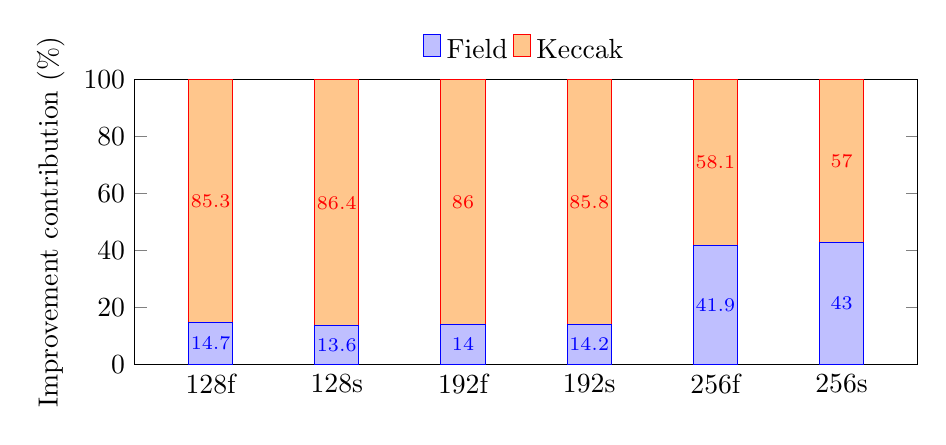
\begin{tikzpicture}
\begin{axis}[
ybar stacked, bar width=16pt,
width=0.95\linewidth, height=5.2cm,
ymin=0, ymax=100, ylabel={Improvement contribution (\%)},
symbolic x coords={128f,128s,192f,192s,256f,256s},
xtick=data, enlarge x limits=0.12,
legend style={at={(0.5,1.02)}, anchor=south, legend columns=2, draw=none},
nodes near coords, every node near coord/.append style={font=\scriptsize},%
]
\addplot+[fill=blue!25] coordinates
{(128f,14.7)(128s,13.6)(192f,14.0)(192s,14.2)(256f,41.9)(256s,43.0)};
\addplot+[fill=orange!45] coordinates
{(128f,85.3)(128s,86.4)(192f,86.0)(192s,85.8)(256f,58.1)(256s,57.0)};
\legend{Field, Keccak}
\end{axis}
\end{tikzpicture}
\caption{Contribution of field arithmetic and Keccak to the overall speedup. Keccak accounts for about 86\% of the improvement in the 128-bit and 192-bit variants, whereas the field contribution increases to about 42\% only in the 256-bit variants.}
\label{fig:decomp}
\end{figure}
